\section{Simuladores para formación médica}
\label{art:medicalsim}

En los últimos años, los simuladores médicos de realidad virtual están tomando una gran importancia en el currículum de los estudiantes, tanto en el campo de la cirugía como en el de otras especialidades \cite{PATEL2017266.e7}. Se puede observar un incremento de su presencia para el entrenamiento de jóvenes especialistas tanto en hospitales como universidades. Estas herramientas proporcionan al usuario un método seguro y efectivo de entrenamiento \cite{simsafety}.

\subsection{Técnicas tradicionales}

Aunque los simuladores están cobrando cada vez más importancia en el ámbito médico, la enseñanza actual se apoya en una gran variedad de métodos de entrenamiento, que permite al médico adquirir las destrezas necesarias, antes de poder enfrentarse a escenarios reales de manera autónoma. 

%\todo{aprendizaje teórico  usanado libros de texto y bases de datos de casos clínicos.(destrezas cognitivas)
%Especialmente en radiologia.  No permiten la adquisición de destrezas no-cognitivas al no permitir interactuar con el paciente.}

El principal método clásico es el aprendizaje teórico, utilizando los libros de texto y la lectura de casos clínicos archivados. 
De esta manera, los profesionales adquieren las destrezas cognitivas necesarias. Aun así, con este método no es posible la adquisición de aquellas habilidades no-cognitivas debido a la ausencia de interacción o práctica que simule un escenario real. 
Para suplir la falta de estas destrezas, la forma de entrenamiento más habitual era la práctica supervisada sobre pacientes reales (\emph{by doing}), donde el estudiante realizaba el procedimiento vigilado y guiado por su tutor. Aunque es el entrenamiento más realista, desde hace décadas se intenta limitar su uso debido a que viene acompañado de situaciones no controladas y de riesgo para el paciente. % \todo{desde la coma suena raro}

Una forma segura de entrenamiento es la utilización de \emph{fantomas}\footnote{Castellanización del término inglés Phantom} \cite{phantomra}. 
Estos \emph{fantomas} son modelos anatómicos hechos con materiales sintéticos que intentan replicar el cuerpo humano y sus propiedades de la forma más fiel posible. En la figura \ref{fig:phantom} se puede ver un ejemplo diseñado para la práctica de ultrasonografía, el \emph{Blue Phantom™}\cite{BluePH}. En ocasiones, estos maniquíes tienen incorporados una serie de sensores que permiten la recogida de métricas de rendimiento. Pero a pesar de que son muy populares, tienen una serie de inconvenientes. Por ejemplo, no son baratos y se crean específicamente para una zona anatómica concreta. No es posible usarlos con otro fin que entrenar el procedimiento para el que fueron diseñados. Además, en determinadas ocasiones el usuario tiene que manipularlos, como puede ser hacer una incisión o realizar una inyección en el \emph{fantoma}, que se traducirá en que el modelo sufrirá desgaste con el tiempo. Por último, destacar que estos modelos representan una única variedad anatómica, haciendo que el médico se enfrente al mismo escenario una y otra vez.
\begin{figure}[ht]
   \centering
    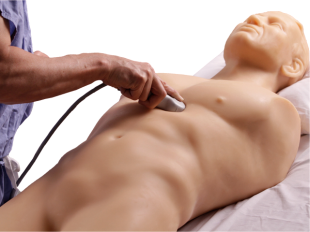
\includegraphics[width=0.8\textwidth]{IMG/fast_trauma.jpg}
    \caption{Maniquí realista para el entrenamiento de ultrasonografía  \emph{Blue Phantom™}\cite{BluePH}. }
   \label{fig:phantom}
\end{figure}

Otra forma de entrenamiento es la utilización de cadáveres \cite{Tsui2007}. De esta manera, el médico puede enfrentarse a casos reales. En este caso, conseguir diferentes variaciones anatómicas es completamente viable y el mismo cadáver puede servir para entrenamientos de diferentes procedimientos. Aun así, los inconvenientes que presentan son bastante evidentes. 
%\todo{Rehaz la última frase. También indicar que la disponibilidad de cadáveres es baja y que no se puede repetir el entrenamiento sobre el mismo paciente. }
La baja disponibilidad de cadáveres y su dificultad para mantenerlos en buenas condiciones, representan sus principales problemas. En ocasiones, los motivos del fallecimiento pueden perjudicar al estado del mismo, o no es posible repetir el mismo entrenamiento en el mismo cuerpo en más de una ocasión. Incluso, existen problemas éticos si se pretende utilizar cadáveres procedentes de condenados a pena de muerte (Visible Human Project \cite{ackerman1998visible}).
Finalmente, uno de los grandes inconveniente de la utilización de cadáveres es que sus tejidos no muestran el mismo comportamiento mecánico que un tejido vivo. Esto puede inducir sesgos en el entrenamiento del profesional médico, debido a que los músculos se vuelven más rígidos después del fallecimiento (efecto conocido como \emph{rigor mortis}).

\subsection{Simuladores de realidad virtual}
\label{art:simulador}

\begin{figure}[ht]
   \centering
    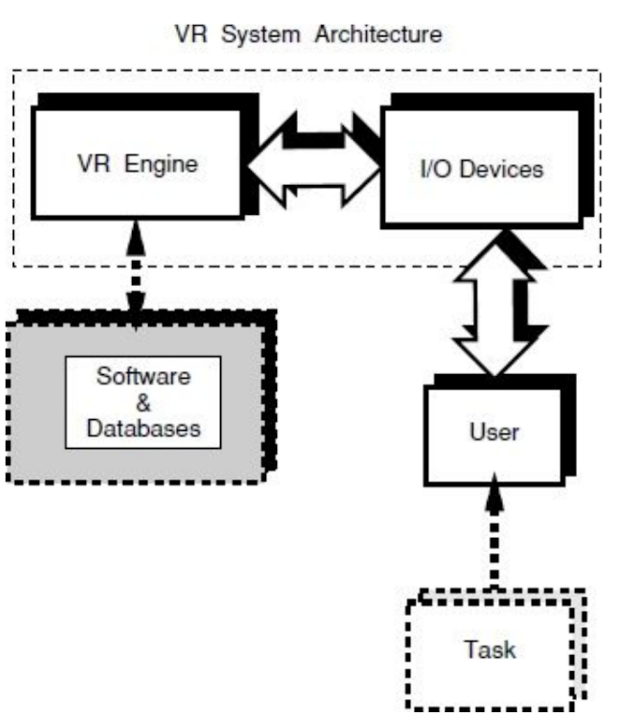
\includegraphics[width=0.5\textwidth]{IMG/VRarq.PNG}
    \caption{Arquitectura para sistemas de \acs{RV} propuesta por \emph{Burdea y Coiffet} \cite{burdea2003virtual}. }
   \label{fig:RVarq}
\end{figure}

%\todo{He metido cambios en la intro y en la sección 1.1 sin el control de cambios. Creo que es peligroso (aunque son muy pequeños). A partir de ahora resaltaré toda la frase aunque el cambio sea mínimo.}
Antes de continuar con la revisión bibliográfica de los simuladores para entrenamiento médico, se va a introducir los conceptos básicos que definen la arquitectura de un sistema de \ac{RV}. %\del{Esto es importante para entender la diferencia que hay entre un simulador de \ac{RV} frente a un simple computador. En esta sección se presenta una propuesta de arquitectura para simuladores de realidad virtual. Esta arquitectura puede ayudar al lector a hacerse una idea de cómo se han construido los simuladores que se presentarán en las siguientes secciones. Además, se utilizará en el capítulo \ref{cap:rasim} como apoyo para explicar el simulador \ac{RASim} y sus diferentes componentes. }
Según \emph{Burdea y Coiffet}\cite{burdea2003virtual}, un sistema de \ac{RV} se puede dividir en cinco componentes tal y como se puede observar en la figura \ref{fig:RVarq}. En ella, además, se puede observar las distintas interacciones que se producen entre estos componentes. Es la relación que existe entre ellos, la que conforma un sistema de \ac{RV}. A continuación, se describirá cada uno de ellos:
\begin{itemize}
    \item Motor de \ac{RV}: este componente se encarga de realizar los cálculos necesarios para simular la escena virtual. Para actualizar el estado de la escena virtual es necesario que se consulte las bases de datos  y actuar según la interacción de los usuario a través de los dispositivos de entrada. El motor generará y mostrará el nuevo estado de la escena a través de los dispositivos de salida (que pueden incluir más de un canal sensorial). Además, es preciso asegurar una tasa de refresco interactiva. El término motor de \ac{RV} no se puede asociar a un computador, sino que se tiene que tratar como una abstracción ya que puede tener múltiples configuraciones hardware, como puede ser un único computador o un sistema distribuido conectado por red.
    \item Dispositivos de \ac{E/S}: este componente lo forman todos los dispositivos que utiliza el usuario en su interacción con el sistema. Es imprescindible para un sistema de \ac{RV}  que se permita la interacción del usuario. Los dispositivos de entrada se encargan de recoger las acciones que realiza el usuario, mientras que los dispositivos de salida muestran la respuesta de la escena virtual a través de los distintos canales sensoriales. Actualmente, estos dispositivos son muy numerosos y diversos.
    \item Componentes software y base de datos: este módulo contiene todas las especificaciones y descripciones que caracterizan el software del sistema. Por una parte, análogamente a una base de datos tradicional, donde se consulta y se recoge información, el resto de módulos consultarán la escena para ejecutar simulación.
    Por otra parte, también es importante nombrar aquellas aplicaciones que se diseñan con el objetivo de guiar y facilitar el entrenamiento. Estas aplicaciones definen como será la interacción del sistema y el usuario a través de la simulación y dan al usuario un motivo para interaccionar con el sistema.%\todo{Rehaz la última frase.}
    \item Usuario: el principal objetivo de la \ac{RV} es presentar al usuario una escena virtual que este perciba como una representación plausible de la realidad. En este sentido, el usuario y la forma en que este percibe e interactúa con el mundo es clave a la hora de diseñar cualquier aplicación \ac{RV}.
    %\del{Es natural que los sistemas se diseñen con el objetivo de que una persona interaccione con ellos. Esta comunicación se realizará a través de los dispositivos de \ac{E/S}}. 
    \item Tareas: por último, son las tareas, objetivos e instrucciones que recibe el usuario cuando va a utilizar el sistema de \ac{RV}, las que dan significado y utilidad a la aplicación. Es lo que le diferencia de ser un computador con periféricos conectados de una plataforma de \ac{RV}.
\end{itemize}


%%%%%%%%% CAMBIO DE SECCION

\subsection{Entrenamiento con simuladores médicos}
\label{art:entrenamiento}


%En anteriores secciones se ha revisado el uso de simuladores en medicina aunque es bien sabido que el uso en otro tipo de contextos no es nuevo. El principal objetivo de estos simuladores es garantizar la seguridad e intentar mejorar el aprendizaje y la respuesta antes errores poco comunes.

En \cite{donaldson2000err}, se cifra en cientos de miles las muertes ocurridas en hospitales estadounidenses como consecuencia de errores médicos, eso sin contar posibles otro tipo de daños a los pacientes que implican gastos económicos. En este libro se planteaba la necesidad de mejorar la formación de los profesionales para evitar este tipo de errores. 
Es necesario también garantizar la seguridad y la intimidad de los pacientes durante el proceso de aprendizaje, lo cual lleva implícito la exigencia ética que representa el propio código deontológico del personal sanitario. 

En el libro \cite{dent2017practical}, se presenta una serie de objetivos que debería cumplir una institución de enseñanza médica al formular el currículum del personal sanitario.
\begin{itemize}
    \item Producir nuevos profesionales sanitarios.
    \item Utilizar los procedimientos médicos modernos.
    \item Cumplir la regulación gubernamental.
    \item Asegurar que los estudiantes puedan completar el curso.
    \item Satisfacer las expectativas de los pacientes.
\end{itemize}

Estos objetivos se enfrentan con una serie de problemas que han impulsado a las instituciones médicas a potenciar el uso de los simuladores.
Por una parte,  desde hace décadas se vienen disminuyendo el tiempo de trabajo para los profesionales en formación, que a la vez reduce el tiempo con pacientes reales. Además, ha habido cambios respecto a que un paciente sea objeto de exploraciones y procedimientos redundantes con la finalidad de entrenar a estudiantes, siendo esta práctica una molestia y un peligro para el paciente. También, hay que añadir que movimientos por los derechos de los animales han hecho restringir el uso de estos con motivos de entrenamiento. Por otra parte, ciertas organizaciones han cambiado sus métodos de evaluaciones con acreditaciones y certificaciones frente a la clásica evaluación basada en el conocimiento exclusivamente.

Otro motivo por el cual es necesario cambiar las formas de aprendizaje de la medicina, es debido a que estas también han evolucionado con el tiempo.
Tradicionalmente, el plan de estudios de la medicina era incremental desde los aspectos más básicos hasta llegar a la especialización. Actualmente la medicina es tan extensa que el contenido del currículum se ha incrementado notablemente. Esto ha hecho que aparecieran escuelas para cada especialidad médica donde el conocimiento médico ha crecido exponencialmente en las últimas décadas y los métodos tradicionales de enseñanza no están completamente adecuados para manejar esa cantidad de material.

Obligados a buscar alternativas para garantizar una exposición clínica variada y completa, junto con el desarrollo de la investigación en el campo de la simulación, los simuladores de \ac{RV} están aumentando su presencia dentro de los procesos de aprendizaje de los futuros médicos.

Frente a un modelo asistencial en la formación de los estudiantes, los simuladores presentan  ventajas educativas que convierten estas herramientas en ideales para enfrentarse a los problemas anteriormente citados. Estas herramientas han demostrado que pueden reducir el tiempo de realización de una tarea, así como el número de errores cometidos y, además, siendo posible diferenciar entre expertos y novatos \cite{Gurusamy08}.

Por otra parte, los simuladores permiten que el estudiante cometa errores sin consecuencias reales. %sin las consecuencias reales que podrían resultar en un entorno con pacientes.
El alumno se puede enfrentar a todo tipo de situaciones, desde las introductorias a las más complicadas donde errar no es crítico. Citando a \cite{ziv2008educacion}: "Los errores son experiencias de aprendizaje y ofrecen grandes oportunidades de mejorar a través del aprendizaje de los mismos". Además, permite que el alumno reciba valoraciones y comentarios en tiempo real. Los simuladores presentan un entorno educativo estandarizado, reproducible y objetivo que permite una evaluación constante de los estudiantes .

A diferencia de los métodos tradicionales anteriormente citados, los simuladores de realidad virtual permiten un entrenamiento más barato y rápido donde los estudiantes pueden mejorar sus habilidades, especialmente las no cognitivas. Mejoras en el rendimiento, nuevos dispositivos de \ac{E/S} y el desarrollo de nuevas técnicas de simulación física, permiten una transferencia efectiva de habilidades del mundo virtual al mundo real \cite{dawereview}.
Habitualmente los simuladores son específicos de cada procedimiento médico, como por ejemplo en \cite{cecil2017advanced} donde se presenta un simulador de cirugía ortopédica. Es también muy habitual encontrar simuladores de cirugía cardiovascular como \cite{korzeniowski2018vcsim3}. En algunos casos se combinan tecnologías de dos o más especialidades para realizar un procedimiento concreto. En  \cite{villard2014interventional} se presenta un simulador de radiología intervencional donde se entrena la habilidad quirúrgica a la vez que se practica el guiado de la aguja a través de una imagen de rayos X.

Pero además, la nueva generación de simuladores no solo se centra en mejorar las habilidades no-cognitivas. Los simuladores permiten entrenar con una gran variabilidad anatómica, desde ejemplos de casos simples hasta los más complejos. Existe la tendencia de permitir el entrenamiento de procedimientos incorporando datos de pacientes que proporcionen ejemplos reales que se puedan encontrar en un futuro \cite{Willaert2012, ZHANG2017599}. 
%\todo{Esta idea queda huérfana aquí. Tienes que desarrollarla. }

El ámbito de los simuladores médicos es muy amplio por lo que, a continuación, la revisión bibliográfica se centrará en las dos especialidades que se van a tratar en la presente tesis.


En cuanto a la especialidad de anestesiología, la anestesia espinal y la epidural son los dos ejemplos más frecuentes dentro de la \ac{RA}, donde se pueden encontrar simuladores específicos \cite{broom2018evaluation}. %Sin embargo, la búsqueda de un simulador de \ac{RA} genérico es más complicada.

En cuanto a la existencia de simuladores de \ac{RA} genéricos, se pueden encontrar algunos ejemplos en la bibliografía. Por ejemplo, \emph{Energid Technologies} ha desarrollado  un simulador al amparo de un contrato con el Ejército de Estados Unidos. El producto final no se ha comercializado al público \cite{lim2008simulation}. Al contrario, un simulador comercial llamado \emph{SAILOR}, se distribuye acompañado de un atlas multimedia de los bloqueos de nervios. Este simulador presenta solo un único modelo de paciente, y su interacción es exclusivamente con el ratón sin ningún tipo de deformación del tejido \cite{Bibin}. 

En un estudio previo al proyecto \ac{RASimAs}, se demostró la aceptación que tendría un simulador para la \ac{RA}. Todos los participantes se mostraron muy receptivos con el trabajo realizado pero se recalcaron la escasez de nervios para bloquear disponibles, la pobre simulación de los ultrasonidos y la ausencia de respuesta háptica \cite{Grottke2009594}.


%\todo{mirar lo que añadió graham}
En cuanto a la enseñanza de radiología diagnóstica, la forma más común de aprender diagnóstico por imagen son los archivos educativos, que son recopilaciones de imágenes médicas de pacientes reales acompañados del historial del paciente. En estos archivos, los estudiantes pueden buscar a través de la gran cantidad de casos bien documentados. Es habitual que cada universidad, hospital o facultad, tengan sus propios repositorios. Además, existen libros donde se pueden consultar recomendaciones y guías \cite{carver2012medical,manualpractico}. 
En la última década, estos recursos se publican cada vez más de manera \emph{online}, donde cualquier radiólogo pueda consultar una enorme base de datos de imágenes de cualquier parte de la anatomía humana \cite{deshpande2017integrated}. 


Actualmente, la educación se ha visto beneficiada por la incorporación de los teléfonos inteligentes en este ámbito. Algunas instituciones han creado aplicaciones donde los estudiantes pueden revisar e investigar los casos almacenados, realizar cuestionarios y mejorar el aprendizaje como es el caso de la aplicación \emph{UBC Radiology} \cite{Spouge2017}. %Estos recursos se encuentran muy presentes en el aprendizaje de los radiólogos noveles.

Complementando la formación teórica, es habitual que se utilicen \emph{fantomas} para entender los principios básicos de radiación sin ningún riegos de dañar un tejido orgánico. Como se ha comentado anteriormente, estos modelos anatómicos son muy caros y no es posible disponer la cantidad necesaria para representar una gran variabilidad anatómica.

Tanto estos recursos como los archivos educativos mantienen el mismo problema: las imágenes registradas son estáticas, y la mayoría de estas imágenes corresponden a imágenes que se presuponen que son correctas y no muestran ningún tipo de fallo. Esto es completamente entendible, ya que al hacer este tipo de recursos se seleccionan aquellas imágenes que no induzcan a error al estudiante. Además, en estos recursos, rara vez aparece un paciente en más de una pose. No es posible ver la misma anatomía u otras partes del mismo sujeto que puedan mostrar diferentes situaciones al estudiante. Aun así, posicionar bien al paciente mientras se realiza el diagnóstico por imagen es imprescindible y necesario que el estudiante domine. 


Por otra parte, las mejoras en el rendimiento de los computadores permiten crear nuevos simuladores que mejoran y reducen el tiempo de aprendizaje de los estudiantes. Un caso notable es el  ProjectionVR$^{TM}$ \cite{shanahan2016student}. Este simulador trata de introducir al usuario dentro de un entorno 3D realista que reproduce una sala de radiología con el objetivo de simular el procedimiento completo. Con datos de pacientes reales digitalizados, el simulador replica un entorno de aprendizaje sin el consecuente riesgo de radiación que significaría exponer a los estudiantes o los pacientes. Aunque la aplicación facilita una cantidad amplia de datos médicos, los imágenes radiográficas que contienen son estáticas y los usuarios no pueden variar o modificar la anatomía del paciente virtual en el simulador. También, hay que destacar la herramienta \emph{medspace.VR} \cite{medspace}. Este simulador proporciona un escenario virtual muy realista que ayuda al usuario a practicar el procedimiento de manera sistemática. Aun así, solo presenta un paciente virtual que únicamente contiene los tejidos de la piel y los huesos, sin ningún otro modelo anatómico interno que pueda ayudar a la correcta identificación de la anatomía del paciente.


Como resultado de todo lo expuesto anteriormente, la tendencia actual demuestra que los simuladores de \ac{RV} se presentan como métodos adicionales de enseñanza con amplios beneficios frente a los métodos tradicionales. Estos simuladores debe ser diseñados y desarrollados teniendo en cuenta una serie de conceptos básicos de aprendizaje que se introducirán  en la sección \ref{art:learning}.
Además, antes de ser incluidas en la formación de nuevos médicos, estas nuevas formas de aprendizaje deben ser validadas y, se debe comprobar si existe una transferencia efectiva de habilidades del simulador a la práctica real. En la sección \ref{art:evaluation}, se presentarán los instrumentos habituales que se utilizan para probar y validar de forma objetiva estas herramientas.








